% executions (for ICS'04)
%
\documentclass[10pt,dvips]{article}
%\documentclass[10pt,twocolumn,dvips]{article}
\usepackage[english]{babel}
\usepackage{epsfig}
%\usepackage{fancyheadings}
%\usepackage[T1]{fontenc}
%\usepackage[latin1]{inputenc}
%\usepackage{twocolumn}
%\usepackage{verbatim,moreverb,doublespace}
%\usepackage{rotate,lscape,dcolumn,array,rotating,latexsym}
%
%\input{epsf}
%
% for somebody (I forget now !)
%\textwidth 175mm
%\textheight 225mm
%\topmargin -4.5mm
%
% for somebody else (I also forget now !)
%\textwidth 6.6in 
%\textheight 239mm
%\topmargin -15mm
%\leftmargin -2.0in
%
% for (IEEE single-column format)
%\textwidth 6.875in
%\textheight 8.875in
%\topmargin -0.6in
%\oddsidemargin 0mm
%\evensidemargin 0mm
%
% for HPCA (IEEE two-column format)
%\textwidth 6.5in
%\textheight 8.875in
%\topmargin -0.4in
%\oddsidemargin 0mm
%\evensidemargin 0mm
%
% for ISPASS
\textwidth 6.5in
\textheight 8.875in
\topmargin -0.4in
\oddsidemargin 0mm
\evensidemargin 0mm
%
%
% turn the following (linespread) on to 1.6 for "double space"
%\linespread{1.6}
%
%
% some publishers want no page numbers for final print
%\pagestyle{empty}
%
\begin{document}
%
%
\title{A Microarchitecture for Parallel Instruction Re-executions}
%
%
\author{
D.A. Morano, D.R. Kaeli\\
Northeastern University\\
{dmorano, kaeli}@ece.neu.edu
}
%
%
% some publishers do not want a data in the final print
\date{1st March 2004}
%
\maketitle
%
% uncomment the following for first page with no page number (for IEEE)
%\thispagestyle{empty}
%
%
\begin{abstract}
%
We describe a microarchitecture oriented towards
the parallel execution and re-execution of many instructions
simultaneously.
In addition to breaking control dependencies, we also allow
for data dependencies to be broken through the speculative
execution of instructions with predicted source operands.
We have redefined the function of the reservation station, or an
issue window instruction slot, providing additional
state and logic that
allows for an instruction dispatched to the station to both
issue for execution when suitable source operands are available
but also to re-issue subsequently when further or later source
operands become available.  We call our adaptation of
this enhanced reservation station an \textit{Issue Station}.
Instructions dispatched to these stations remain associated
with the station for the duration of the instruction's lifetime
within the execution window of the machine (until the instruction
is retired being either committed or abandoned).
New instructions are only dispatched to an Issue Station when the
previously dispatched instruction to the station is retired.

Rather than determine instruction dependencies at 
instruction issue, we dynamically determine instruction data
dependencies as the instructions are executing (or re-executing).
We employ time ordering tags with both Issue Stations and
all operands for data dependency management within the machine.
By using these time ordering tags, dispatched instructions
are ordered with respect to each other and all active operands
being transferred among machine components.  All operands
are also tagged as they are transferred among the various machine 
components.  All instructions are dispatched in-order but are
allowed to repeatedly issue out-of-order as conditions that
might signal the need for an execution or re-execution occur.
All instructions are retired in-order.

We present simulation data for the microarchitecture that
focuses on exploring the dynamics of the machine
operation associated with instruction execution, re-execution,
and operand forwarding and acquisition.
The data presented serves to characterize the machine
with varying numbers of different machine components configured.
As expected, the performance of the machine, as measured with
Instructions Per Cycle (IPC), generally increases with increasing
machine resources but also shows where an increase in 
the number of
components do not improve performance for a given 
configuration, or may even decrease performance due to
excessive contention for a resource.
%%DAVE: WE NEED NUMBERS HERE (XX IPC, XX% better than an XYZ machine).
IPC results for the SpecInt-2000 benchmark suite ranged
from about 5.8 to about 9.0 for
a machine with the approximate hardware resources as a
current superscalar machine.
For similar machine resources, we performed about 15\% better than
a similar proposed microarchitecture that shares some of
our instruction and operand handling techniques.
%
\end{abstract}
%
%
%\vspace{-0.25in}
\section{Introduction}
%\vspace{-0.15in}
%
Although many high performance applications today
can be parallelized at the source code level 
and executed on clustered systems,
there are and will continue
to be requirements for achieving the highest performance
on single threaded program codes.
We attempt to target this application problem space
through the extraction of instruction level parallelism (ILP).
However, 
high execution performance through ILP
extraction has not generally been achieved even though
large amounts of ILP are present in integer sequential programs
codes.
Several studies into the limits of instruction level 
parallelism have shown that there is 
a significant amount of parallelism within
typical sequentially oriented single-threaded programs
(e.g., SpecInt-2000).  
The work of researchers including 
Lam and Wilson~\cite{Lam92},
Uht and Sindagi~\cite{Uht95},
Gonzalez and Gonzalez~\cite{Gon97}
have shown that there exists a great amount of instruction level
parallelism that is not being exploited by any existing
computer designs.

A basic challenge 
is to find program parallelism and then allow execution to occur
speculatively, in parallel, and out of order over 
a large number of instructions.
Generally, this is achieved by introducing multiple
execution units into the microarchitecture where each unit
can operate as independently as possible and in parallel, thus
achieving increased execution instructions per clock (IPC).
It is also usually very desirable to support legacy instruction
set architectures (ISAs) when pursuing high IPC. 
For this reason, we want to explore a
microarchitecture that is suitable for implementing any ISA.

Microarchitectures that have employed the
use of multiple execution units are the Multiscalar-like
processors~\cite{Sohi95,sundararaman97multiscalar},
the SuperThreaded processor model~\cite{tsai96superthread},
and
the Parallel Execution Window processor model~\cite{kemp96pew}.
Other microarchitecture proposals such as the MultiCluster machine
model by 
Farkas et al.~\cite{farkas97multicluster} are also in this category.
In particular, the Multiscalar processors have
realized substantial IPC speedups over conventional superscalar
processors, but they rely on compiler participation in their
approach.

Another attempt at realizing high IPC was done by
Lipasti and Shen on their Superspeculative
architecture~\cite{Lip97}.  They achieved an IPC of
about 7 with conventional hardware assumptions but
also by using value prediction.
Nagarajan proposed a {\em Grid Architecture} of ALUs
connected by an operand network~\cite{Nag01}.  
This has some similarities to our work.
However, unlike our work, their microarchitecture
relies on the coordinated use of the compiler along with
a new ISA to obtain higher IPCs.
Also, Morano and Uht~\cite{morano02high,uht02realizing}
have introduced a microarchitecture for extraction of
high ILP that features both
a large number of parallel execution units and a more flexible
mechanism for managing concurrent control and data dependencies.
Their microarchitecture can also be applied to any existing ISA.

Our goal is to design a microarchitecture
that features the benefits of the Superspeculative 
microarchitecture and its ability to break data
dependencies through value prediction, with the flexibility
of managing a large number of independently executing and re-execution
instructions as in the microarchitectural proposal above by Uht et al.  
But we also wanted to retain the approximate machine resource
sizes of some of the
more conventional microarchitectures like the
MIPS R10000~\cite{yeager96r10000} and R12000, 
the Compaq Computer 
Alpha processor 21264~\cite{Kessler98,leibholz97alpha},
and the latest Intel Pentium processor~\cite{hinton01pentium}.
Our new microarchitectural model can
be applied to any existing ISA.  
The microarchitecture can speculatively execute a large
number of instructions in parallel without strictly adhering to
the data dependency chains in the program.  This makes it
suitable and attractive for handling sequential codes.
We call our microarchitecture \textit{OpTiFlow}, which
is an abbreviation for Operand Time Flow.
The name reflects that program-time-ordered instruction operands
are a significant feature of the microarchitecture.

%% DAVE: Summarize performance data here....
We present IPC results from the machine for idealized memory and branch
prediction that serve to provide a first characterization of
this new microarchitecture.  
Our IPC results ranged from about 5.8 to about 9.0 for
a machine with the approximate hardware resources as a
conventional superscalar today.  

The rest of this paper is organized as follows.
Section 2 gives a description of our microarchitecture.
Section 3 provides some characterization and performance 
results for our microarchitecture through the simulated
execution of benchmark programs.
We summarize in section 4.
%
%% DAVE: Was this the name that we arrived at?  Give the reader some name
%% to grasp on to.
%\vspace{-0.25in}
\section{The OpTiFlow Microarchitecture}
%\vspace{-0.15in}
%
In the following subsections we present an
overview of our microarchitecture called OpTiFlow, followed by details
of its more novel major components.
We also discuss some of the algorithms used to manage
the handling of operands and the enforcement of
operand dependencies for correct program order commitment.
%
%\vspace{-0.25in}
\subsection{Microarchitecture Overview}
%\vspace{-0.15in}
%
At a high-level, our microarchitecture resembles many existing
and past microarchitectures that employ reservation stations
or issue windows along with multiple execution function units.
The handling of main memory, and the cache hierarchy 
through the L1 instruction and L1 data caches are all
conventional and similar to existing microarchitectures.
Some of the additional major components of our
microarchitecture are a
load-store-queue (LSQ) component, an architected register file,
structures that closely resemble reservation stations or issue
window slots, and rather conventional execution function units.
The most novel aspect of our microarchitecture is how we
handle instruction issue for execution and re-execution.
In order to efficiently handle instruction issue and re-issue,
we have redefined the function of a machine structure
resembling a reservation station with additional state and control
logic.  
Our new structure is called 
an \textit{issue station} (IS).
Like other machines with reservation stations, we dispatch 
decoded instructions from the fetch unit to these Issue Stations
when one or more of them are empty (available for dispatch) or 
becoming empty on the next clock cycle.  
Instructions are dispatched in-order.
As expected, the number of instructions dispatched in any 
given clock cycle is
the lesser of the number of ISs available and the
dispatch width (as counted in numbers of instructions).
In our microarchitecture, instructions can be dispatched to
ISs with or without initial input source operands.
Operand dependency determination is not done before
either instruction dispatch (to an issue station) nor
before instruction operation issue to a function unit for
execution.
All operand dependencies are determined dynamically through
snooping after instruction dispatch.
This is explained more later.

Figure \ref{fig:overview} shows a high-level block diagram
of our microarchitecture showing the major instruction execution components.
The memory hierarchy, as well as details of the instruction fetch
unit, are not shown as they are similar to those of existing
machines.
%
\begin{figure}
\centering
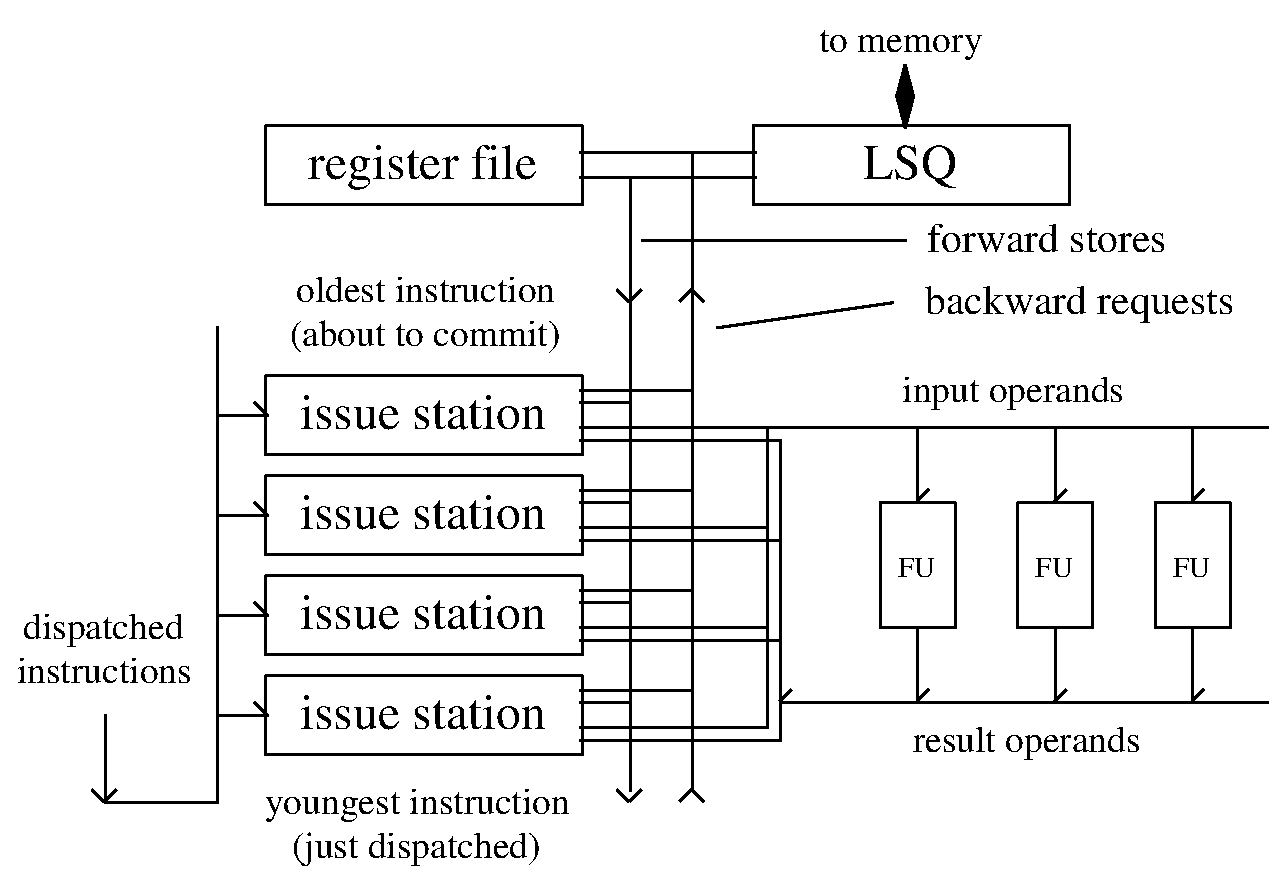
\epsfig{file=figure1.eps,width=6.0in}
\caption{{\em High-level block diagram of our microarchitecture.} 
Issues stations are shown on the left and various function
units on the right.  An architected register file and a
load-store-queue is shown at the top.
Bidirectional operand request and forwarding buses are shown
vertically oriented (to the right of the Issue Stations).
Buses to transport an instruction operation and its source operands
to the function units are also shown. 
Likewise buses to return result operands are present.}
\label{fig:overview}
\end{figure}
%
In the top left of the figure is the architected register file.
Since all operand renaming is done within the Issue Stations,
only architected registers are stored here.
In the top right is the load-store-queue.
The lower right shows (laid out horizontally) a set of function units.
Each function unit (three are shown in this example)
is responsible for executing a class of
instructions and generally has independent pipeline depths.
The function unit pipelining allows for new operations to arrive
on each successive clock cycle while generating new results on
each cycle.
Table \ref{tab:futypes} shows the types of function units
currently implemented and the default number of pipeline stages
present in each unit.
Note that instructions not associated with a function unit
are executed within the issue station itself.  This currently
includes all control-flow change instructions as well as load-store
instructions.  
The lower left shows (laid out vertically) the set of
Issue Stations (four are shown in this example)
that may be configured into an implementation of
the machine.
The ISs are all identical without regard to 
instruction type.  This allows for all instructions to be
dispatched in-order to the next available ISs 
without further resource restrictions or management.
%
%
\begin{table}[p]
\begin{center}
\caption{{\em Default execution function unit types and pipeline stages.}
Both the number of function units of each type and the pipeline depths 
of each
can be configured within our microarchitectural simulation framework.
The far right column shows some numbers of function unit
types that might be implemented in a typical machine.}
\label{tab:futypes}
\vspace{+0.1in}
\begin{tabular}{|l|c|c|}
\hline 
FU type&pipeline depth&typical number\\
\hline
IALU&1&8\\
\hline
IMULT&7&2\\
\hline
IDIV&12&2\\
\hline
FADD&4&2\\
\hline
FCMP&4&2\\
\hline
FCVT&3&1\\
\hline
FMULT&4&2\\
\hline
FDIV&12&1\\
\hline
FSQRT&18&1\\
\hline
\end{tabular}
\end{center}
\end{table}
%
%

In the center of Figure \ref{fig:overview},
running vertically, are two buses shown.
These bidirectional and multi-master buses 
form the means to request and forward operands
among the ISs, register file, and LSQ.
Each of these buses is actually a parallel set of identical buses
that are statistically multiplexed to increase operand transfer
bandwidth.  
Other bus arrangements are possible (some fairly complicated by
comparison).  
Further, separate bus fabrics for handling
different types of operands is also possible.
One of these buses is used by ISs
for requesting source operands and
has been termed a \textit{backwarding request} bus.
The name is derived from the fact that requested operands should
only be satisfied by those instructions that lie in the program-ordered
past from the instruction requesting the operand.
The other bus is used for forwarding operands to younger instructions
and is often termed the \textit{forwarding} bus.
Operands need to be forwarded from older dispatched
instructions to younger dispatched instructions.
The arrows on the buses show the direction of intended travel
for operands (or operand requests) that are placed on each bus
respectively.  Although the register file and LSQ only receive
operand requests on the backwarding request bus, the ISs
both receive and transmit requests from their connections to that
bus.  Likewise, although the register file and LSQ only transmit
operands on the operand forwarding bus, the ISs
both receive and transmit on their connections to that bus.

Finally, unidirectional buses are provided to interconnect
the ISs with the function units.
One bus serves to bring instruction
operations along with their source operands from an issue
station to a function unit.
The other bus returns function unit results back to its
originating issue station.
Again these buses are generally multiple identical buses in
parallel to allow for increased transfer bandwidth.
It is assumed that all buses carry out transfers at the same
clock rate as the rest of the machine including the execution
function units.

Collectively, all of the components discussed in this section
(and shown in 
Figure \ref{fig:overview}) we term the \textit{execution window}.
This term is adapted from a similar functional definition in prior
work~\cite{uht02realizing}.
The number of ISs in
any given machine implementation roughly corresponds to the
number of elements of a reorder buffer or a register update unit
in a more conventional machine.
The number of function units somewhat corresponds to the
issue width of machines with multiple, and more general, execution pipelines.
%
%\vspace{-0.25in}
\subsection{Issue Stations}
%\vspace{-0.15in}
%
The Issue Stations provide the most significant distinction of this
microarchitecture from most others.
Still, our issue station and its operational philosophy
is very similar to that used by 
Uht et al.~\cite{uht03levo}, which itself was very similar to
their previous work~\cite{uht02realizing}.
Our Issue Stations can be thought of as being 
reservation stations~\cite{Tom67} but
with additional state and logic added to them that allows
for dynamic operand dependency determination as well as
for holding a dispatched instruction (its decoded form) 
until it is ready to be
retired.  This differs from conventional reservation stations
or issue window slots in that the instruction does not free
the station once it is dispatched to a function unit.
Also, unlike reservation stations, but like an issue window slot,
the instruction operand from an issue station may be dispatched
to different function units (not just one that is strictly
associated with the reservation station).

The state associated with an issue station can be grouped into
two main categories.  There is state that is relevant to
the instruction itself, and secondly there is state that is
related to the operands of that instruction (both source and
destination operands).
The state associated with the instruction itself has to do
with the ordering of this instruction in relation to the other
instructions that are currently in the execution window.
The remainder of the state consists of one or more input
source operands and one or more output destination operands.
All operands regardless of type and whether source or destination
occupy a similar structure within an issue station, termed an
\textit{operand block}.
The operand blocks all have connectivity to both the
operand request and forwarding buses as well as to the FU
issue and result buses.
More detail on these operand blocks and operand management
is provided in the next section.

The state that is primarily associated with the instruction itself
consists of the following :
%
%% DAVE: MAYBE NOT FOR THIS PAPER, BUT IT MIGHT BE NICE TO SHOW A 
%% FSM DIAGRAM FOR EXECUTION STATE.
\begin{itemize}
\vspace{-0.10in}
\item{instruction address}
\vspace{-0.10in}
\item{instruction operation}
\vspace{-0.10in}
\item{execution state}
\vspace{-0.10in}
\item{path ID}
\vspace{-0.10in}
\item{time ordering tag}
\vspace{-0.10in}
\item{instruction predication information}
\vspace{-0.10in}
\end{itemize}   
%
The \textit{instruction operation} is derived from the decoded
instruction and specifies the instruction class and other
details needed for the execution of the instruction.
This information may consist of subfields and is generally ISA
specific.
The \textit{instruction address} and \textit{predicate} state
are only used when dynamic predication~\cite{morano02predication}
is done within the
microarchitecture.
The \textit{path ID} value is used when dynamic multipath
execution is done.
The \textit{time tag} value is used to order this instruction
with respect to all others that are currently within the execution
window of the machine.
The \textit{execution state} value consists of a set of
bits that guide the execution of the instruction through
various phases.  Some of this state includes :
%
\begin{itemize}
\vspace{-0.10in}
\item{in the process of acquiring source operands for first time}
\vspace{-0.10in}
\item{execution is needed}
\vspace{-0.10in}
\item{in the process of executing (waiting for result from FU)}
\vspace{-0.10in}
\item{at least one execution occurred}
\vspace{-0.10in}
\item{a result operand was requested by another issue station}
\vspace{-0.10in}
\item{a result operand is being forwarded}
\vspace{-0.10in}
\end{itemize}   
%
In addition to guiding the operation of the issue station,
many of these state bits are used in the commitment determination
for this issue station.

A simplified block diagram of our issue station is shown in 
Figure \ref{fig:issuestation}.
%
\begin{figure}
\centering
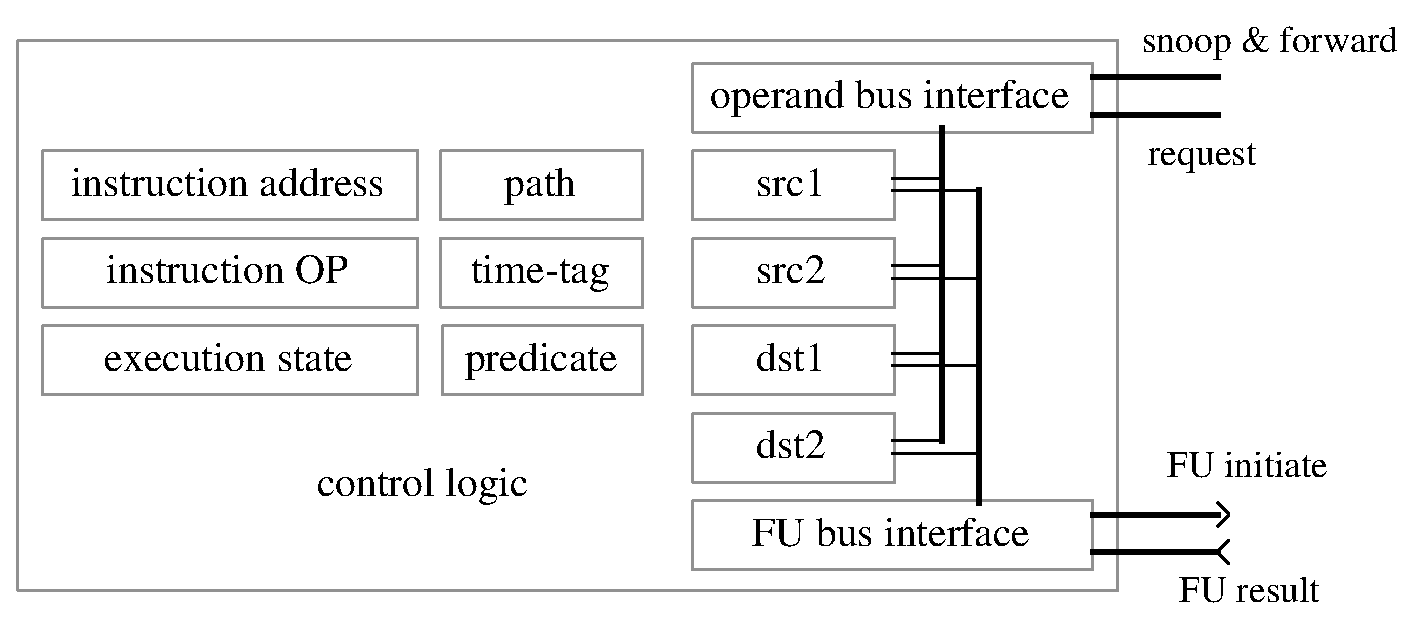
\epsfig{file=figure2.eps,width=6.0in}
\caption{{\em High-level block diagram of our Issue Station.} 
The major state associated with an Issue Station is shown:
four operand blocks (two source and two destination)
and its four bus interfaces, grouped
according to bus function into two major logic blocks.}
\label{fig:issuestation}
\end{figure}
%
The state associated primarily with just the instruction is
shown on the left of the block diagram while the operand blocks
and their connectivity to the various buses is shown on the
right.  
In this example, a total of four operand blocks are shown, labeled:
\textit{src1}, 
\textit{src2}, 
\textit{dst1}, 
and \textit{dst2}.
The number of source and destination operand blocks that are
used for any given machine is ISA dependent.
Some ISAs require up to five source operands and up to three destination
operands (usually for handling double precision floating point 
instructions).
Generally, any operand in the ISA that can cause a separate
and independent data dependency (a unique dependency name)
requires a separate operand block for it.
No additional operand block is needed when dynamic predication
is performed since its state would be included as
part of the general issue station state mentioned previously.
%
%
%\vspace{-0.25in}
\subsection{Operands}
%\vspace{-0.15in}
%
At least three types of instruction operands may be identified
for most microarchitectures: 
1) register, 2) memory, and 3) predicate operands.
Register and memory operands are similar enough that
they share an identical operand block
As mentioned previously, the state for managing predicate
operands is always just included with the general state within
an issue station.
The state that may be associated with the handling of
dynamic predicates is more complicated than that for
just register or memory operands, and it is dependent
on the dynamic predication scheme that might be employed.
The specifics of predicate operands is not elaborated on
further in this paper.

The register state within an operand block consists of :
%
\begin{itemize}
\vspace{-0.10in}
\item{type of operand}
\vspace{-0.10in}
\item{path ID}
\vspace{-0.10in}
\item{time ordering tag}
\vspace{-0.10in}
\item{sequence number}
\vspace{-0.10in}
\item{address}
\vspace{-0.10in}
\item{size}
\vspace{-0.10in}
\item{previous value}
\vspace{-0.10in}
\item{value}
\vspace{-0.10in}
\end{itemize}   
%
The operand \textit{type}, \textit{path ID}, and \textit{time ordering tag}
serve
an analogous purpose as those fields do within an issue station,
except that these fields now apply specifically to this particular
operand rather than to the instruction as a whole.

The \textit{address} field differs
depending on the type of the operand.
For register operands, the address would be
the name of the architected register.
All ISA architected registers are typically provided a
unique numerical address.  These would include the
general purpose registers, any status or other non-general
purpose registers, and any possible ISA (architected) predicate registers
(like those in the iA-64 ISA~\cite{intel99ia,schlansker00epic}.
For memory operands, the identifying address is just the
programmer-visible architected memory address of the corresponding
memory value.

Although the time ordering tag uniquely identifies the issue station
that forwarded the operand, it does not indicate information about
a particular instance of that operand being forwarded.
The \textit{sequence number} is used to disambiguate different
instances of an operand forwarded with the same time tag.
This is only needed when more elaborate forwarding interconnection fabrics
are used that allow an operand to either get duplicated in flight
or to pass and overtake another operand in real time.
The sequence number is not used in the present work.

The \textit{size} is only used for memory operands and holds
the size of the memory reference in bytes.
The \textit{value} holds the present value of the operand,
while the \textit{previous value} is only used for destination
operands and holds the value that the operand
had before it may have been changed by the present instruction.
The previous value is used in two possible circumstances.
First, it is used when dynamic predication is
employed and the effects of the present instruction need to be
squashed (if and when its enabling predicate becomes false.)
It is also used when a forwarded operand with a specific
address was incorrect 
and there is no expectation that a later instance
of that operand with the same address will be forwarded.
This situation occurs when addresses for memory operands are
calculated but are later determined to be incorrect.
An operand with the old address is forwarded with the previous
value to correct the situation.
Figure \ref{fig:operand} shows a simplified block diagram of
an operand block.
%
\begin{figure}
\centering
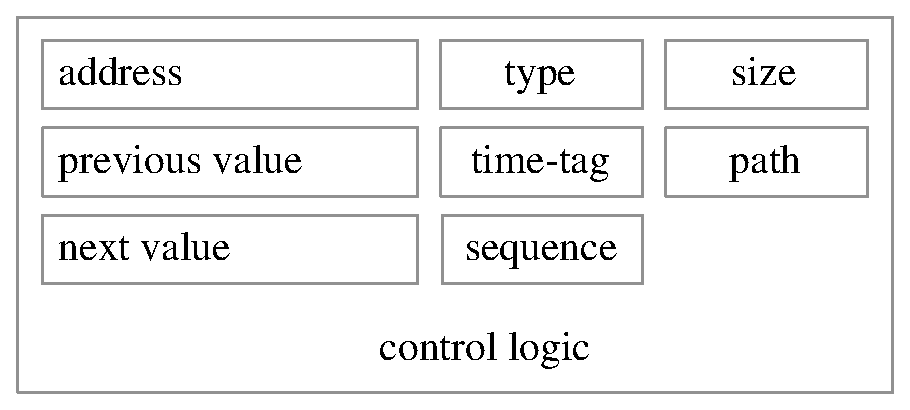
\epsfig{file=figure3.eps,width=3.0in}
\caption{{\em Block diagram of an Operand Block.} 
Each Operand Block holds an effectively renamed 
operand within the Issue Stations.
Several operand blocks are employed within each Issue Station
depending on the needs of the ISA being implemented.
The state information maintained for each operand
is shown.}
\label{fig:operand}
\end{figure}
%

From the state that is maintained for each operand, it can be seen
that 
all operands originating from an issue station
are uniquely named within the
execution window of the machine.
Unique operand names consist of components :
%
\begin{itemize}
\vspace{-0.10in}
\item{type of operand}
\vspace{-0.10in}
\item{path ID}
\vspace{-0.10in}
\item{time tag}
\vspace{-0.10in}
\item{address}
\vspace{-0.10in}
\end{itemize}   
%
When needed, a specific instance of a unique operand
is further disambiguated by the \textit{sequence number} element.
In effect,
a full renaming of
all operands is realized for all instructions
in flight in the machine.  
All false dependencies are now avoided.
There is no need to limit instruction dispatch or to limit speculative
instruction execution due to a limit on the number of non-architected
registers used for holding temporary results (or renaming registers).
Through this renaming scheme
no physical register renaming is needed at instruction dispatch
or issue time.  
And finally, we have completely obviated the need for
register update units, reorder buffers, future files, or other physical 
renaming register structures or mechanisms.
%
%
%\vspace{-0.25in}
\subsection{Dependency Ordering}
%\vspace{-0.15in}
%
Rather then calculating instruction dependencies at instruction
dispatch or issue time, we allow instructions to begin
the process of executing (possibly with incorrect operands)
while also providing for instructions to
dynamically determine their own correct
operand dependencies.
The mechanism used for this dynamic determination of
operand dependencies is to provide a special tag that
conveys the program-ordered relative time of the origin of
each operand.
As previously shown,
a time ordering tag is associated
with the operational state of both Issue Stations and operands.
These time ordering tags are small
integers and uniquely identify the relative position of an instruction
or an operand in program ordered time.
Typically, time tags take on small positive values with
a range approximately equal to the 
number of Issue Stations implemented in
the machine.  Thus the number of bits used is approximately
the log base two of the number of Issue Stations.

A time tag value of zero is associated with the
issue station holding the instruction that is next ready
to retire (the one that was dispatched the furthest in the past).
Later dispatched instructions take on successively higher
valued tags.
As Issue Stations retire, the time tag registers in all
ISs and operand blocks are decremented by the
number of Issue Stations being retired.
Committed operands can thus be thought of as taking on
negative valued time tags.  Negative valued tags can also have
microarchitectural applications but those are beyond the
scope of this present work.
Operands that are created by instructions that have executed
(the outputs of the instruction) take on
the same time tag value as its originating issue station.  
By comparing time tag values with each other, the relative
program-ordered time relationship is determined.
We next discuss
how operands are transferred from one
issue station to another, while enforcing the necessary
true program dependencies for proper execution.
%
%
%\vspace{-0.25in}
\subsection{Operand Forwarding and Snooping}
%\vspace{-0.15in}
%
Operands resulting from the execution of instructions
are transmitted forward for use by waiting instructions.
Whether an operand value is broadcast, multicast, or more narrowly
directed forward
is determined by the nature of the operand forwarding interconnection
fabric being employed.

As expected, when operands are forwarded, not only is the 
address of the operand
and its value sent, but also its time tag, a sequence number (if needed),
and its path ID 
(for
those microarchitectures using multipath execution).
%% DAVE: CONSIDER ELIMINATING THE DISCUSSION OF SEQUENCE NUMBERS.
This information is used by subsequent 
dispatched instructions 
(later in program order time)
to determine if
the operand should be {\em snarfed}~\footnote{Snarfing entails snooping
buses, and when the desired address value is detected, 
the associated data value is read.}.
Snarfed input operands generally trigger either execution
(if the instruction has not executed yet)
or re-execution.

The information associated with each operand that is
transmitted from one IS to a subsequent IS
is referred
to as a {\em transaction}, and generally consists of :
%
\begin{itemize}
\vspace{-0.10in}
\item{transaction type}
\vspace{-0.10in}
\item{operand type}
\vspace{-0.10in}
\item{path ID}
\vspace{-0.10in}
\item{time tag of the originating instruction}
\vspace{-0.10in}
\item{sequence number}
\vspace{-0.10in}
\item{address}
\vspace{-0.10in}
\item{data value for this operand}
\vspace{-0.10in}
\end{itemize}   
%
This above information is typical of both
register and memory operand transactions.
The use of the \textit{operand type} transaction field 
for operand names may not be
necessary depending on how the different operand types
are transferred among instructions.
For example, if different request and forwarding buses are
provided for different operand types, the type of the operand
would not need to be transmitted on the bus fabric itself.
The \textit{transaction type} field is used to further
identify the type of transaction.  
For example, if requests for operands and the forwarding of
actual operands share a common interconnection fabric, then
this field is used to distinguish them.
Further, other transaction types can be used to indicate that
a previously forwarded operand is no longer valid.
%% DAVE WHAT DOES THIS SENTENCE MEAN??
%% Operand referrals among Issue Stations is also possible.
A number of management mechanisms are possible but
these are beyond the scope of this present work.

True flow dependencies are enforced through the continuous snooping of
these transactions by each dispatched instruction, residing in an issue
station, that receives the transaction.
Each issue station
will snoop all operands that are received by it.
Some 
interconnection fabrics may be devised such that
transactions are only sent to those instructions that primarily
lie in future program-ordered time from the originating instruction,
but the general mechanism presented 
still handles even the general (and worst)
case when transactions are simply broadcast to all other Issue Stations.  

A simplified diagram of the logic used for operand snooping
is shown in Figure \ref{fig:source}.
The {\em time-tag}, and
{\em value} registers are reloaded with new values on each snarf,
while the
{\em path} and
{\em instr time-tag} are only loaded when an instruction is
dispatched.
The {\em address} register is either loaded at instruction
dispatch or may be loaded during instruction execution
(for example by load/store instructions).
%
\begin{figure*}
\centering
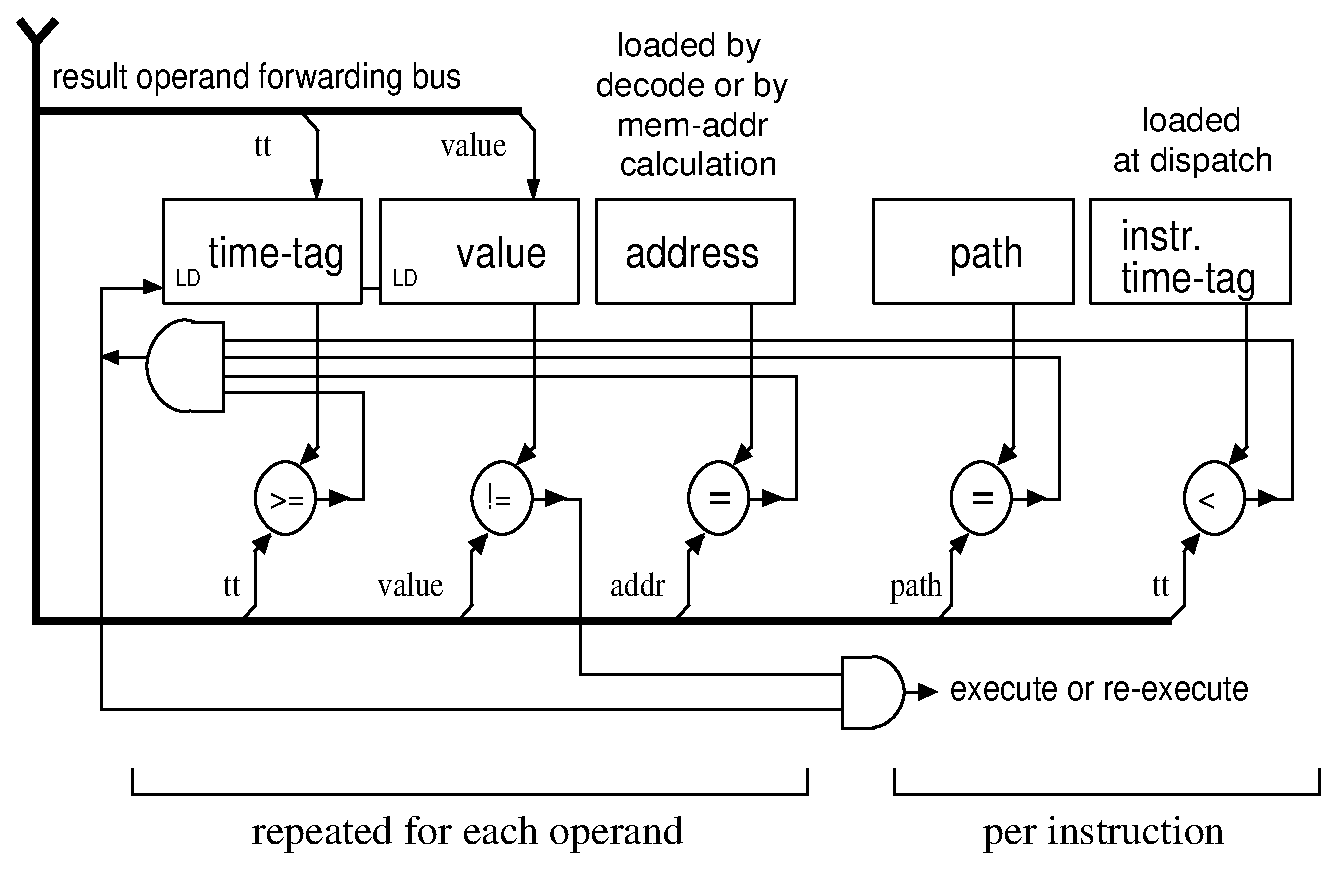
\epsfig{file=figure4.eps,width=6.0in}
\caption{{\em Snooping for operand updates.} 
The registers and snooping
operation of one of several possible source operands is shown.
This logic would reside in an operand block within an issue slot.
Just one operand forwarding bus is shown being snooped but
typically several forwarding buses are snooped simultaneously.}
\label{fig:source}
\end{figure*}
%
If the
path ID and the identifying address of the operand matches any of
its current input operands, the logic also checks
if the time tag value of the operand being snooped
is less than its own assigned time tag
and greater than or equal to the time tag value of the last
operand that it snarfed, if any.  
When sequence numbers are used (not shown in the diagram),
an additional check is performed.
If the snooped data value is
different than the input operand data value that the instruction 
already has, a re-execution of the instruction is initiated.
This simple rule allows for the dynamic discovery of
all program dependencies during instruction execution while 
also allowing for maximum concurrency to occur.
%
%
%\vspace{-0.25in}
\section{Experimental Results}
%\vspace{-0.15in}
%
In this section we present experimental results from simulation
of the machine presented.
These results are primarily presented to characterize the
nature and potential performance of the machine with a few major
components varied.
Our machine implements the Alpha~\cite{Bannon95} instruction set.
All benchmarks were compiled using the native OSF1 (Digital Unix)
compiler under the OSF1 operating system 
using standard compiler optimization,
and targeted for execution on the OSF1 operating system.
System calls from the programs are emulated within the simulator,
but otherwise all other instructions are handled
within the simulated microarchitecture as presented previously.
The simulator itself is very detailed in its operation for
all of the major components of the microarchitecture.

We use ten of Spec2000 integer benchmarks to evaluate the potential
of this microarchitecture. 
For all simulations, the first 300 million instructions of each
benchmark program is executed without regard for functional machine
consequences.  
This is done to step the programs past their initialization
phases.
A short sequence of instructions are then
executed to warm up the functional simulator.
The next 400 million instructions are then
functionally executed on the machine.

The machine used in these simulations
employed a simple operand forwarding fabric consisting of
several buses in parallel.  The number of buses was set high
enough to accommodate as many operands in a single clock cycle as
needed to be forwarded.
One clock period is used to traverse the buses.
Since we wanted to focus on the novel aspects of our machine,
we have relaxed restrictions on instruction fetch and
the memory hierarchy.
These conditions allow us to focus more directly on the
machine operations associated with instruction execution, and
operand forwarding and acquisition.
We idealized the memory hierarchy
by having all data references and instruction fetches hit in 
the L1 caches with a one cycle
access latency.
Further, we idealized instruction fetch by using a 100\% accurate
branch predictor.
By default, the number of pipeline stages in each type of
of function unit, along with the number of the units of that
type, is given in Table~\ref{tab:futypes}.
The default number of function units provide similar
execution resources for integer programs running on an
eight issue wide machine such as the Alpha EV8~\cite{jain01eveight}.
Further, for these present characterizations the dispatch width
of the machine is set large enough to also allow for the maximum
number of instructions to be dispatched in each clock cycle where
Issue Stations are available.
Other numbers of components, machine widths, or latencies are
specified with the individual data results.
Neither dynamic predication nor multipath execution
is currently being performed with this machine.
%
%
%\vspace{-0.25in}
\subsection{Comparison With Other Microarchitectures}
%\vspace{-0.15in}
%
Although an exact comparison between different microarchitectures
is not possible, a rough comparison between microarchitectures
using roughly the equivalent hardware resources is attempted.
We compare three machines, a conventional superscalar,
the Levo microarchitecture ~\cite{uht03levo}, and our OpTiFlow
microarchitecture.
The Levo machine has 256 reservation station-like structures
(similar to our Issue Station structures)
enabling it to execute 256 instruction in parallel.
The conventional superscalar has both 256 reservation stations
and 256 re-order buffer entries serving a similar purpose.
We compare these with 256 issue stations in our microarchitecture.
The conventional and OpTiFlow machines both have 16 integer
ALU FUs and additional FUs similar as those listed in Table~\ref{tab:futypes},
while the Levo machine has 64 general purpose execution units
(capable of executing any type of instruction).
Pipeline depth for the integer FUs and the Levo execution 
units for integer instructions is one.  Other pipeline depths
for non-integer instructions are similar and are listed
for the conventional and OpTiFlow machines in Table~\ref{tab:futypes}.
All other parameters are set similarly or idealized appropriately
to match all machine conditions as closely as possible.
The conventional microarchitecture was configured and simulated
using the Simplescalar MASE framework~\cite{Austin97}
while the Levo results are from ~\cite{uht03levo}.
The IPC results from the three machines are given in Table~\ref{tab:compare}.
%
\begin{table}[p]
\begin{center}
\caption{{\em Comparison of IPC performance with other machines.}
IPC performance of a MASE machine and a Levo machine is
shown with that of OpTiFlow.}
\label{tab:compare}
\vspace{+0.1in}
\begin{tabular}{|l||r|r|r|}
\hline 
 & MASE & Levo & OpTiFlow \\
\hline

\hline
bzip2&
3.2 & 12.9 & 9.5 \\

\hline
crafty&
3.4 & 9.9 & 11.9 \\

\hline
eon&
1.9 & NA & 7.9 \\

\hline
gcc&
3.2 & 9.8 & 11.8 \\

\hline
gzip&
2.6 & 8.5 & 12.7 \\

\hline
parser&
2.4 & 9.1 & 12.1 \\

\hline
perlbmk&
2.9 & NA & 10.3 \\

\hline
twolf&
2.7 & NA & 11.3 \\

\hline
vortex&
2.9 & 10.2 & 11.3 \\

\hline
vpr&
2.0 & NA & 13.0 \\

\hline
\end{tabular}
\end{center}
\end{table}
%
The harmonic mean IPCs for the conventional and OpTiFlow machines,
over all benchmarks, are 2.6 and 10.7 respectively.  
The harmonic mean IPCs for
the Levo and OpTiFlow machines, over their common benchmarks,
are 10.0 and 11.5 respectively.
Clearly the Levo and OpTiFlow machines are much more structured
for handling the large instruction execution parallelism,
exploitable from the program codes.
The OpTiFlow harmonic mean IPC is about 15\% higher than
that of the Levo machine while using only 16 integer ALU FUs
compared with the 64 general purpose execution units for the Levo machine.
%
%
%\vspace{-0.25in}
\subsection{Varying the Number of Issue Stations}
%\vspace{-0.15in}
%
One of the more obvious aspects of our microarchitecture
that contributes to the amount of ILP
that can be extracted from the programs is the number of Issue Stations
implemented.
Here we simulate five machines with
varying numbers of Issue Stations.
We present two data sets here.  
We began by configuring a machine with  
8 integer ALUs and then extended this to 16 ALUs.
A machine  
with 128 Issue Stations and eight integer ALU FUs resembles
a typical machine in development today.
The taget design point is centered around a next generation
machine that has an issue width of 16 rather than 8.

The IPC results for all 
benchmarks along with the harmonic mean 
is shown for this first data set (8 integer ALU function units)
in Table \ref{tab:iwsize8ipc}.
The percent of IS stalls due to function unit unavailability
is shown in Table \ref{tab:iwsize8waits}.
The average percent of instruction executions that are 
actually re-executions ranged from about 1.2\% for the configuration
with 16 Issue Stations to about 2.2\% for 256 Issue Stations.
Although only 8 integer FUs are employed, IPCs for a program
can be greater than 8 since other instructions are executed
either within the issue station itself or by other FU types.
Notice that the highest IPC performance is not achieved with
the largest number of Issue Stations but rather with the configuration
with 64 Issue Stations (having a harmonic mean of 8.0).  
The IPC starts to decrease due to
the destructive contention for function units (actually the integer
ALU units).
The reason for this can be seen in the IS stall 
data (Table~\ref{tab:iwsize8waits}) where the percent of
requests by the Issue Stations for the integer ALU is over
60\% and 80\% for the cases of 128 and 256 Issue Stations
respectively.
%
\begin{table}[p]
\begin{center}
\caption{{\em IPC performance for varying numbers of
Issue Stations.}
All machines had 8 integer ALU FUs with varying ISs from 16 to 256.}
\label{tab:iwsize8ipc}
\vspace{+0.1in}
\begin{tabular}{|l||r|r|r|r|r|}
\hline 
{ISs}& 16 & 32 & 64 & 128 & 256 \\
\hline

\hline
bzip2&
5.1 & 7.7 & 7.4 & 5.8 & 3.6 \\

\hline
crafty&
4.9 & 7.7 & 8.1 & 7.3 & 6.1 \\

\hline
eon&
4.2 & 6.6 & 8.3 & 8.0 & 6.0 \\

\hline
gcc&
5.2 & 8.0 & 8.0 & 6.8 & 6.7 \\

\hline
gzip&
5.2 & 8.0 & 8.1 & 7.6 & 5.6 \\

\hline
parser&
5.1 & 7.6 & 8.0 & 7.3 & 7.6 \\

\hline
perlbmk&
5.1 & 8.1 & 7.2 & 5.9 & 3.6 \\

\hline
twolf&
4.8 & 7.5 & 7.7 & 7.3 & 5.2 \\

\hline
vortex&
5.3 & 8.9 & 9.0 & 8.1 & 5.5 \\

\hline
vpr&
4.7 & 7.5 & 8.7 & 8.4 & 6.5 \\

\hline
H-MEAN&
4.9 & 7.7 & 8.0 & 7.1 & 5.3 \\

\hline
\end{tabular}
\end{center}
\end{table}
%
%
\begin{table}[p]
\begin{center}
\caption{{\em Percentage FU-request stalls
with varying numbers of Issue Stations.}
All machines had 8 integer ALU FUs with varying ISs from 16 to 256.}
\label{tab:iwsize8waits}
\vspace{+0.1in}
\begin{tabular}{|l||r|r|r|r|r|}
\hline 
{ISs}& 16 & 32 & 64 & 128 & 256 \\
\hline

\hline
bzip2&
4.8 & 29.0 & 64.4 & 82.1 & 91.4 \\

\hline
crafty&
4.8 & 28.2 & 63.3 & 81.4 & 90.6 \\

\hline
eon&
17.9 & 33.7 & 55.5 & 74.1 & 85.2 \\

\hline
gcc&
5.1 & 29.9 & 63.7 & 82.1 & 89.3 \\

\hline
gzip&
4.0 & 27.4 & 64.9 & 82.2 & 91.3 \\

\hline
parser&
3.5 & 33.4 & 66.3 & 92.0 & 89.9 \\

\hline
perlbmk&
4.4 & 24.5 & 63.2 & 82.0 & 91.6 \\

\hline
twolf&
5.6 & 28.2 & 63.7 & 81.4 & 91.2 \\

\hline
vortex&
3.3 & 18.3 & 58.9 & 79.1 & 89.8 \\

\hline
vpr&
7.3 & 27.6 & 59.6 & 78.4 & 89.0 \\

\hline
\end{tabular}
\end{center}
\end{table}
%

The IPC results for the 
second configuration (16 integer ALU function units)
are shown in Table \ref{tab:iwsize16ipc}.
The percent IS stalls due to function unit unavailability
is shown in Table \ref{tab:iwsize16waits}.
These results show a similar trend found in the previous set
except that the IPC numbers are higher.
However, the configuration with 64 Issue Stations is still
the highest performing design with a harmonic mean of 14.5.
The average percent of instruction executions that are re-executions
range from about 0.9\% to 1.8\% 
when we vary the number of ISs from 16 to 256 respectively.
%
\begin{table}[p]
\begin{center}
\caption{{\em IPC performance for varying numbers of
Issue Stations.}
All machines had 16 integer ALU FUs with varying ISs from 16 to 256.}
\label{tab:iwsize16ipc}
\vspace{+0.1in}
\begin{tabular}{|l||r|r|r|r|r|}
\hline 
{ISs}& 16 & 32 & 64 & 128 & 256 \\
\hline

\hline
bzip2&
5.3 &  10.1	&  16.0 	&  13.0	&   9.5 \\

\hline
crafty&
5.1 &   9.2	&  14.8	&  14.4	&  11.9 \\

\hline
eon&
4.3 &   6.8	&   9.5	&  10.3	&   7.9 \\

\hline
gcc&
5.4 &  10.1	&  15.6	&  14.9	&  11.8 \\

\hline
gzip&
5.3 &  10.3	&  16.6	&  14.9	&  12.7 \\

\hline
parser&
5.2 &   9.9	&  14.7	&  14.8	&  12.1 \\

\hline
perlbmk&
5.4 &  10.2	&  15.8	&  13.4	& 10.3 \\

\hline
twolf&
5.0 &   9.2	&  14.5	&  14.1	& 11.3 \\

\hline
vortex&
5.4 &  10.2	&  17.9	&  15.7	& 11.3 \\

\hline
vpr&
4.9 &   8.7	&  13.8	&  15.2	& 13.0 \\

\hline
H-MEAN&
5.1 & 9.3 & 14.5 & 13.9 & 11.0 \\

\hline
\end{tabular}
\end{center}
\end{table}
%
%
\begin{table}[p]
\begin{center}
\caption{{\em Percentage IS stalls for FUs
with varying numbers of Issue Stations.}
All machines had 16 integer ALU FUs with varying ISs from 16 to 256.}
\label{tab:iwsize16waits}
\vspace{+0.1in}
\begin{tabular}{|l||r|r|r|r|r|}
\hline 
{ISs}& 16 & 32 & 64 & 128 & 256 \\
\hline

\hline
bzip2&
0.0 & 3.1 & 22.9 & 64.5 &  82.4 \\

\hline
crafty&
0.0 & 4.8 & 25.2 & 63.0 & 81.6 \\

\hline
eon&
16.7 & 29.0 & 44.6 & 62.6 & 78.6 \\

\hline
gcc&
0.0 & 3.0 & 26.5 & 62.8 & 82.0 \\

\hline
gzip&
0.0 & 2.3 & 23.2 & 65.0 & 82.6 \\

\hline
parser&
0.0 & 3.4 & 32.5 & 65.9 & 83.1 \\

\hline
perlbmk&
0.1 & 2.9 & 22.8 & 63.2 & 82.2 \\

\hline
twolf&
1.3 & 6.2 & 27.1 & 63.6 & 82.4 \\

\hline
vortex&
0.1 & 2.2 & 14.1 & 59.1 & 79.8 \\

\hline
vpr&
3.1 & 7.9 & 27.0 & 59.4 & 78.8 \\

\hline
\end{tabular}
\end{center}
\end{table}
%
%
%\vspace{-0.25in}
\subsection{Varying the Number of Integer ALU Function Units}
%\vspace{-0.15in}
%
Next, we present data characterizing the effect of the
number of integer FUs available.
We are only focusing on the integer ALU FU type
because for the integer benchmarks that we are executing,
almost no other FUs are used.
The only modest exception to this is made by the EON and VPR programs,
which possess a noticeable percentage of floating point instructions.
These programs have a slightly lower IPC than the others
due to the number of floating point FUs in our configuration
(one or two, reference Table \ref{tab:futypes}).

Tables \ref{tab:nialu16ipc} 
and \ref{tab:nialu16waits} 
show the results
for a machine with a window size of 16 (16 Issue Stations) and various
numbers of integer ALU function units.  
%
\begin{table}[p]
\begin{center}
\caption{{\em IPC performance for varying integer ALU FUs.}
All machines had 16 ISs with varying integer ALU FUs from 2 to 16.}
\label{tab:nialu16ipc}
\vspace{+0.1in}
\begin{tabular}{|l||r|r|r|r|}
\hline 
{IALUs}& 2 & 4 & 8 & 16 \\
\hline

\hline
bzip2&
2.1 & 3.9 & 5.1 & 5.3 \\

\hline
crafty&
2.3 & 3.9 & 4.9 & 5.1 \\

\hline
eon&
2.9 & 4.0 & 4.2 &  4.3 \\

\hline
gcc&
2.4 & 4.1 & 5.2 & 5.4 \\

\hline
gzip&
2.2 & 3.8 & 5.2 & 5.3 \\

\hline
parser&
2.2 & 3.9 & 5.1 & 5.2 \\

\hline
perlbmk&
2.4 & 4.1 & 5.1 & 5.4 \\

\hline
twolf&
2.2 & 3.9 & 4.8 & 5.0 \\

\hline
vortex&
2.4 & 4.7 & 5.3 & 5.4 \\

\hline
vpr&
2.4 & 3.9 & 4.7 & 4.86 \\

\hline
H-MEAN&
2.3 & 4.0 & 4.9 & 5.1 \\

\hline
\end{tabular}
\end{center}
\end{table}
%
%
\begin{table}[p]
\begin{center}
\caption{{\em Percentage IS stalls for FUs
with varying numbers of integer ALU FUs.}
All machines had 16 ISs with varying integer ALU FUs from 2 to 16.}
\label{tab:nialu16waits}
\vspace{+0.1in}
\begin{tabular}{|l||r|r|r|r|}
\hline 
{IALUs}& 2 & 4 & 8 & 16 \\
\hline

\hline
bzip2&
66.2 & 32.5 & 3.3 & 0.0 \\

\hline
crafty&
65.2 & 31.3 & 4.6 & 0.0 \\

\hline
eon&
51.7 & 26.9 & 17.4 & 16.7 \\

\hline
gcc&
64.8 & 33.3 & 4.4 & 0.0 \\

\hline
gzip&
67.0 & 34.5 & 4.0 & 0.0 \\

\hline
parser&
67.4 & 35.8 & 3.5 & 0.0 \\

\hline
perlbmk&
64.3 & 28.8 & 4.4 & 0.1 \\

\hline
twolf&
65.5 & 30.6 & 5.6 & 1.3 \\

\hline
vortex&
63.3 & 26.4 & 3.3 & 0.1 \\

\hline
vpr&
62.2 & 29.8 & 7.3 & 3.1 \\

\hline
\end{tabular}
\end{center}
\end{table}
%
As expected, IPC increases when we increase the
number of integer
ALUs.
Note that for the case where there are 16 integer ALU function
units, there are seldom IS stalls due to function
unit contention.  
This is expected, as the total number of instructions executing
simultaneously never exceeds 16 (for this set of results) since
the number of Issue Stations configured was 16.
The exceptions are with the EON and VPR programs
that are contending for the limited number of floating point units.
The EON program places almost one third of its FU requests
for the floating point multiply unit and about 
about one eighth for the floating point multiply unit.
The VPR program places about one eleventh of its FU requests
for the floating point add unit with some on the other
floating point units also.
The average percent of instruction executions that are re-executions
ranges from about 2.2\% to 0.9\% 
when varying from 2 to 16 integer ALU FUs respectively.
%
%
%\vspace{-0.25in}
\subsection{Varying the Number of Integer ALU Pipeline Stages}
%\vspace{-0.15in}
%
Here we explore the effect of FU pipeline depth on the IPC
performance.
On machines with 128 ISs and 16 integer ALU FUs,
we vary the integer ALU FU pipeline depth from 1 to 4.
The IPC results are shown in Table \ref{tab:lialu16ipc}.
%
\begin{table}[p]
\begin{center}
\caption{{\em IPC performance for varying integer ALU FU pipeline stages.}
All machines had 128 ISs and 16 integer ALU FUs but with varying 
integer ALU FU pipeline stages of from 1 to 4.}
\label{tab:lialu16ipc}
\vspace{+0.1in}
\begin{tabular}{|l||r|r|r|r|}
\hline 
{stages}& 1 & 2 & 3 & 4 \\
\hline

\hline
bzip2&
13.0 & 11.9 & 11.8 & 12.1 \\

\hline
crafty&
14.4 & 13.7 & 13.1 & 12.7 \\

\hline
eon&
10.3 & 10.6 & 10.6 & 10.3 \\

\hline
gcc&
14.9 & 13.9 & 13.2 & 12.3 \\

\hline
gzip&
14.9 & 13.8 & 13.3 & 14.3 \\

\hline
parser&
14.8 & 14.0 & 13.8 & 12.8 \\

\hline
perlbmk&
13.4 & 12.6 & 11.9 & 10.7 \\

\hline
twolf&
14.1 & 13.3 & 13.0 & 12.7 \\

\hline
vortex&
15.8 & 15.0 & 15.1 & 14.6 \\

\hline
vpr&
15.2 & 14.6 & 14.2 & 13.6 \\

\hline
H-MEAN&
13.9 & 13.2 & 12.9 & 12.5 \\

\hline
\end{tabular}
\end{center}
\end{table}
%
%
As expected the IPC consistently decreases across all programs
as the integer ALU FU pipeline depth is increased.
The IPC decreased about 10\% when going from a single stage
pipeline depth to 4 stages.
Perhaps contrary to intuition, the average percent
IS stalls for all FUs decreases, rather than increases,
as the integer ALU FU pipeline depth is increased.
The average percent of IS stalls decreases from 62.9\% to 53.5\%
for pipeline depths of 1 to 4, respectively.
This is due to the fact that at present the issue station does not 
attempt to re-issue an instruction operation
(request an FU), while that issue station is already executing 
an instruction (is waiting for the FU result).
%
%
%\vspace{-0.25in}
\section{Summary}
%\vspace{-0.15in}
%
We have described a new microarchitecture that combines
some of the features of conventional superscalar microarchitectures
along with those of a value-predicting microarchitecture.
We have enabled a new kind of
{\em flexible} instruction execution parallelism
and a specific dependency enforcement mechanism
of more elaborate research microarchitectures while maintaining
the approximate size and complexity constraints of current or near term
machines.
This has been achieved while still maintaining binary program
compatibility with
existing ISAs (and the Alpha ISA in particular).

The percent of executions that are re-executions does not
exceed about 3.0\% since we presently do not allow
an issue station to initiate a new execution request
before an existing execution request is completed.
Allowing multiple simultaneous execution requests
to be issued
from a single Issue Station is one direction for
future research.  We are also interested in the power characteristics
of using re-execution versus a more centralized hazard resolution
mechanism.

We have presented data that partially characterizes our
microarchitecture and shows its potential for exploiting
ILP from sequential programs.  
Our partially idealized IPC results ranged from about 5.5 to 9.0 for
machine configurations with resources similar to those of
current or next generation superscalar processors,
and were about 15\% better than those of a
more complicated proposed microarchitecture that employs similar
instruction and operand handling but with more execution units
than we employed.
In the final version of this
paper we plan to expand upon our data presentation by including
simulations that consider both correct memory behavior and
control flow prediction.
%
\bibliographystyle{latex8}
\bibliography{executions}
%
\end{document}
%
%
%
